\section{Auswertung}
\label{sec:Auswertung}

\subsection{Vorbereitung und technische Daten}

\begin{table}
    \centering
    \caption{Technische Daten.}
    \label{tab:techDaten}
    \begin{tabular}{l l c l}
        \toprule
        Medium          & Größe                 & Variable      & Wert                                      \\
        \midrule
        Flüssigkeit     & Dichte                & $\rho$        & $\SI{1.15}{\gram\per\cubic\centi\meter}$  \\
                        & Schallgeschwindigkeit & $c_\text{L}$  & $\SI{1800}{\meter\per\second}$            \\
                        & Viskosität            & $\eta$        & $\SI{12e-3}{\pascal\second}$              \\
        Prisma          & Schallgeschwindigkeit & $c_\text{P}$  & $\SI{2700}{\meter\per\second}$            \\
                        & Vorlaufstrecke        & $l$           & $\SI{30.7}{\milli\meter}$                 \\
        Strömungsrohr   & Innendurchmesser      & $d_\text{i}$  & $\SI{10}{\milli\meter}$                   \\
                        & Außendurchmesser      & $d_\text{a}$  & $\SI{15}{\milli\meter}$                   \\
        \bottomrule
    \end{tabular}
\end{table}

Das verwendete Prisma hat drei verschiedene (Prisma-)Winkel $\theta$, unter denen die Strömung in den Rohren untersucht wird. 
Der daraus resultierende Doppler-Winkel $\alpha$ wird über 
\begin{equation*}
    \alpha=\SI{90}{\degree}-\arcsin \Bigl(\sin \theta \cdot \frac{c_\text{L}}{c_\text{P}}\Bigr)
\end{equation*}
berechnet. Die Kenndaten $c_\text{L}$ und $c_\text{P}$ sind in Tabelle \ref{tab:techDaten} zu finden.

Die Werte für die Winkel sind in Tabelle \ref{tab:Winkel} aufgeführt.
\begin{table}
    \centering
    \caption{Prisma- und Doppler-Winkel.}
    \label{tab:Winkel}
    \begin{tabular}{c c}
        \toprule
        Prisma-Winkel $\theta$ & Doppler-Winkel $\alpha$ \\
        \midrule
        $\SI{15}{\degree}$ & $\SI{80.064}{\degree}$ \\        
        $\SI{30}{\degree}$ & $\SI{70.529}{\degree}$ \\
        $\SI{45}{\degree}$ & $\SI{61.874}{\degree}$ \\        
        \bottomrule
    \end{tabular}
\end{table}

\subsection{Die Strömungsgeschwindigkeit in Abhängigkeit des Doppler-Winkels}

\begin{table}
    \centering
    \caption{Messwerte der Frequenzverschiebungen in Abhängigkeit des Prisma-Winkels~$\theta$.}
    \label{tab:1Mess}
    \begin{tabular}{c c c c c c c}
        \toprule
            & \multicolumn{3}{c}{$\Delta \nu_\text{max}\,/\,\si{\hertz}$} & \multicolumn{3}{c}{$\Delta \nu_\text{mean}\,/\,\si{\hertz}$} \\
        \cmidrule(lr){2-4} \cmidrule(lr){5-7}
        rpm & $\SI{15}{\degree}$ & $\SI{30}{\degree}$ & $\SI{45}{\degree}$ & $\SI{15}{\degree}$ & $\SI{30}{\degree}$ & $\SI{45}{\degree}$ \\
        \midrule
        2000 &  90 & 120 & -105 &  49 &  73 & -61  \\
        2800 &  94 & 235 & -145 &  61 & 134 & -85  \\
        3600 & 135 & 375 & -220 &  85 & 208 & -122 \\
        4400 & 200 & 555 & -330 & 110 & 293 & -165 \\
        5200 & 290 & 820 & -470 & 146 & 415 & -232 \\
        \bottomrule
    \end{tabular}
\end{table}

Die aufgenommenen Messwerte sind in Tabelle \ref{tab:1Mess} zu finden. 
Der Rechner für die Datenaufnahme zeigt jeweils zwei Werte für die Frequenzverschiebung an: Zum einen die maximale, zum 
anderen die gemittelte Frequenzdifferenz. 
Beide Werte sind für die Auswertung aufgenommen worden, um vergleichen zu können, welche eine stärkere experimentelle Aussage zulassen. 

Die Zentrifugalpumpe gibt hierbei ihre Umdrehungen pro Zeiteinheit in $\mathrm{rpm}$ (\textit{revolutions per minute}) an; es wird erwartet, dass die Umdrehungszahl 
proportional zur Strömungsgeschwindigkeit der Flüssigkeit ist. 
In den Abbildungen \ref{fig:exp15}, \ref{fig:exp30} und \ref{fig:exp45} sind die Frequenzverschiebungen gegen die Umdrehungszahl aufgetragen. 
In den nebenstehenden Abbildungen \ref{fig:theo15}, \ref{fig:theo30} und \ref{fig:theo45} ist jeweils die Frequenzverschiebung 
gegen die Strömungsgeschwindigkeit $v$ aufgetragen, die über die Formel 
\begin{equation*}
    \Delta \nu=2 \nu_0 \frac{v}{c} \cos \alpha
\end{equation*}
berechnet wird. Verwendet wird eine $\SI{2}{\mega\hertz}$-Sonde, deshalb ist $\nu_0=\SI{2}{\mega\hertz}$. 

Aufgrund des als proportional angenommenen Zusammenhangs zwischen der Drehzahl der Pumpe und der Strömungsgeschwindigkeit 
wird angenommen, dass die Messpunkte in den Graphiken \ref{fig:15}, \ref{fig:30} und \ref{fig:45} einen ähnlichen Verlauf haben. 

\begin{figure}
    \centering
    \begin{subfigure}{0.48\textwidth}
        \centering
        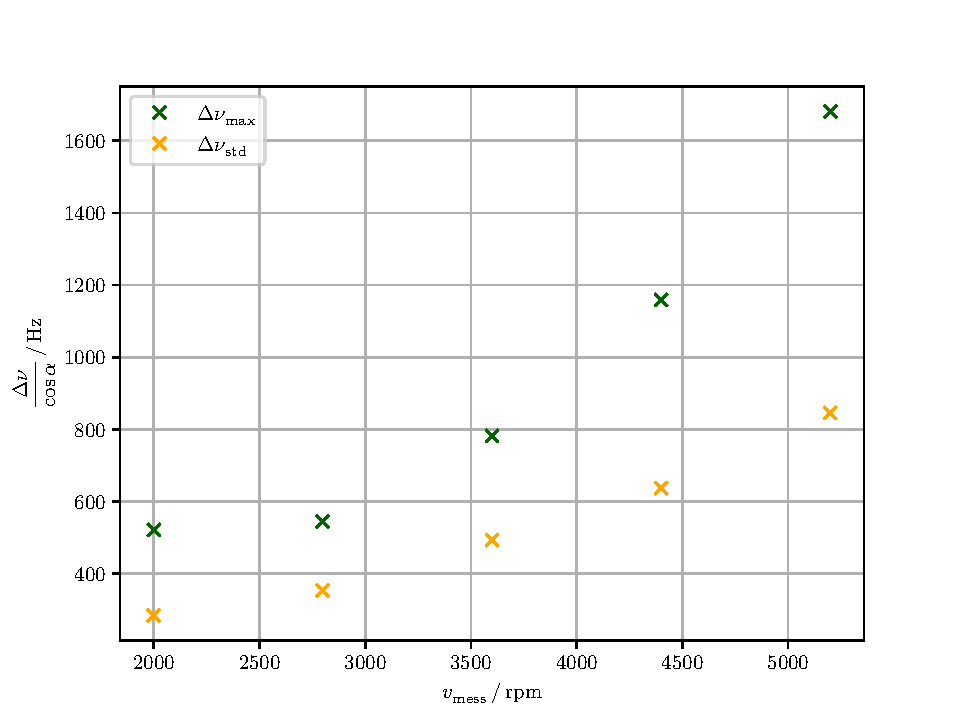
\includegraphics[height=5.5cm]{plots/15_2.pdf}
        \caption{Mit der Geschwindigkeit, die durch die Zentrifugalpumpe gegeben wird.}
        \label{fig:exp15}
    \end{subfigure}
    \begin{subfigure}{0.48\textwidth}
        \centering
        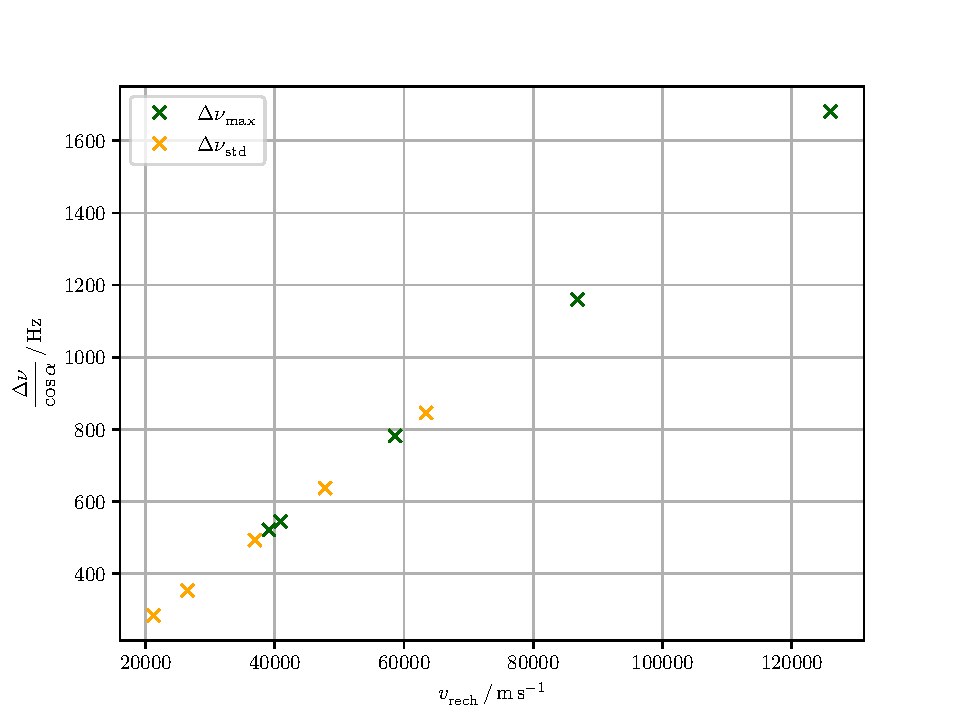
\includegraphics[height=5.5cm]{plots/15_1.pdf}
        \caption{Theoretisch berechnete Strömungsgeschwindigkeit.}
        \label{fig:theo15}
    \end{subfigure}
    \caption{Graphiken zum Prisma-Winkel $\theta=\SI{15}{\degree}$.}
    \label{fig:15}
\end{figure}
\begin{figure}
    \centering
    \begin{subfigure}{0.48\textwidth}
        \centering
        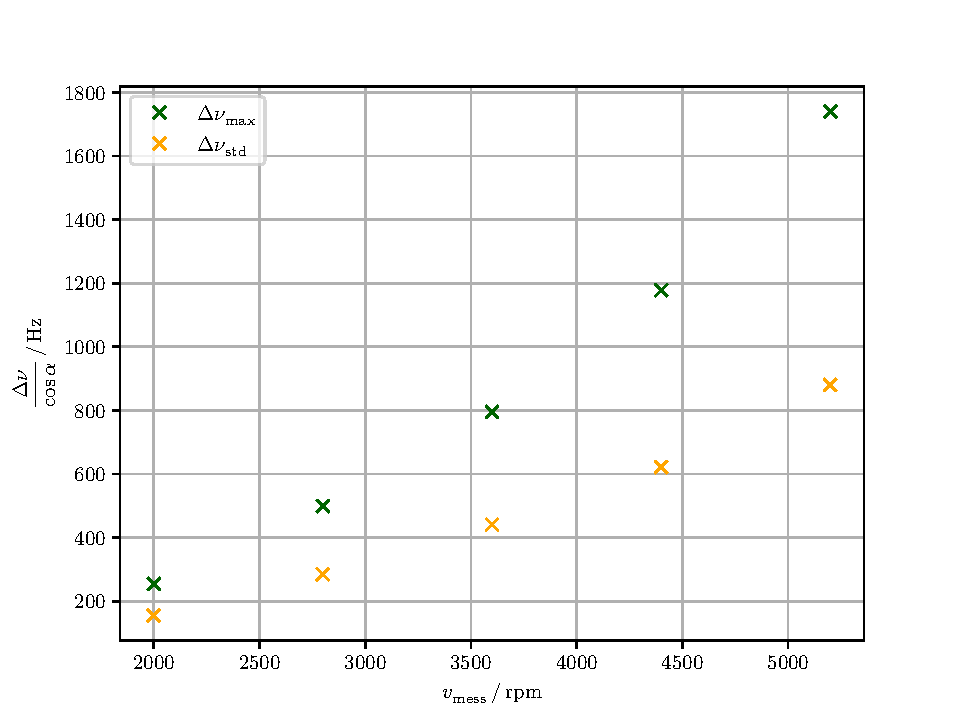
\includegraphics[height=5.5cm]{plots/30_2.pdf}
        \caption{Mit der Geschwindigkeit, die durch die Zentrifugalpumpe gegeben wird.}
        \label{fig:exp30}
    \end{subfigure}
    \begin{subfigure}{0.48\textwidth}
        \centering
        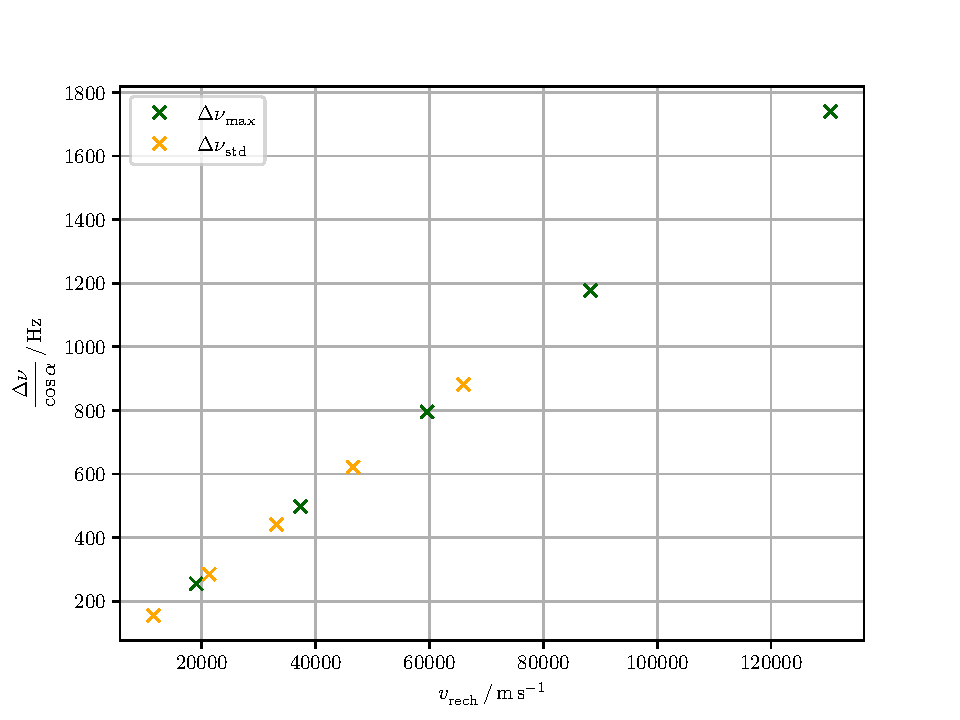
\includegraphics[height=5.5cm]{plots/30_1.pdf}
        \caption{Theoretisch berechnete Strömungsgeschwindigkeit.}
        \label{fig:theo30}
    \end{subfigure}
    \caption{Graphiken zum Prisma-Winkel $\theta=\SI{30}{\degree}$.}
    \label{fig:30}
\end{figure}
\begin{figure}
    \centering
    \begin{subfigure}{0.48\textwidth}
        \centering
        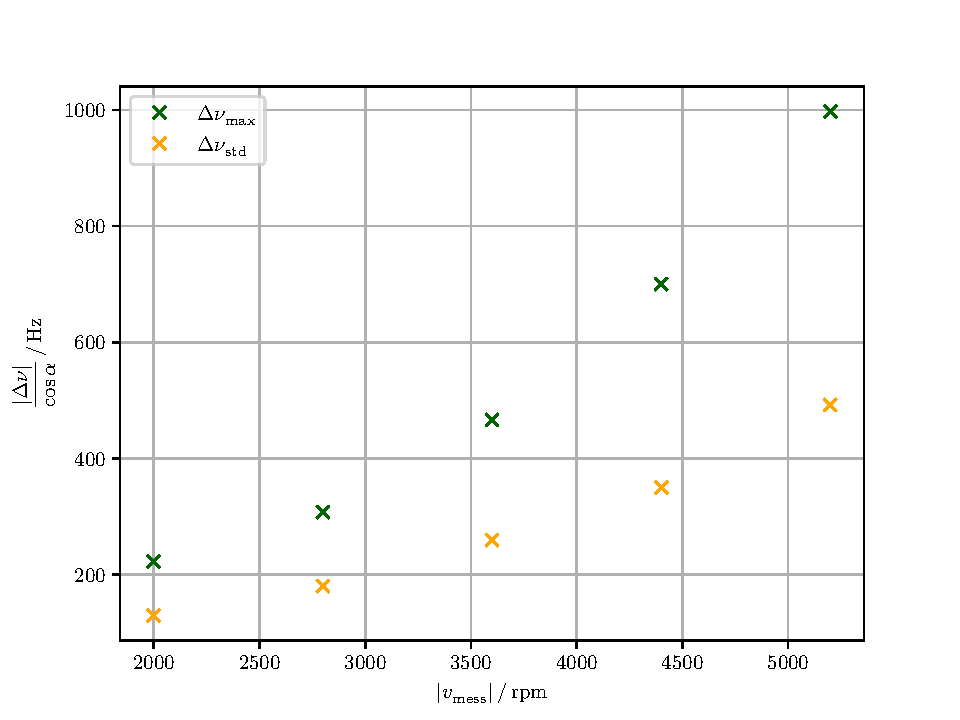
\includegraphics[height=5.5cm]{plots/45_2.pdf}
        \caption{Mit der Geschwindigkeit, die durch die Zentrifugalpumpe gegeben wird.}
        \label{fig:exp45}
    \end{subfigure}
    \begin{subfigure}{0.48\textwidth}
        \centering
        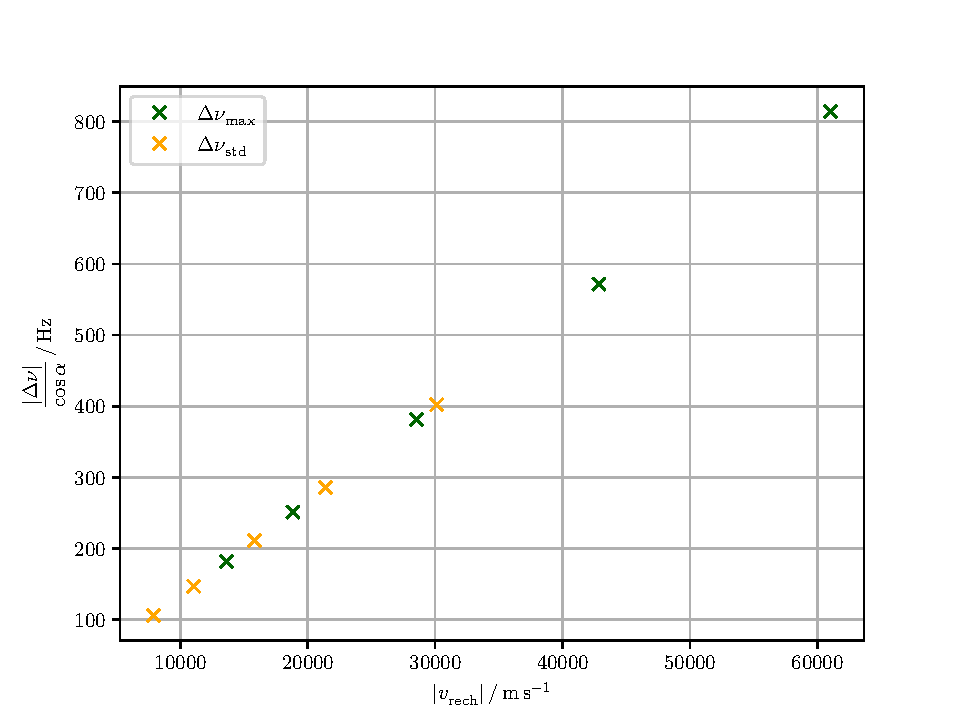
\includegraphics[height=5.5cm]{plots/45_1.pdf}
        \caption{Theoretisch berechnete Strömungsgeschwindigkeit.}
        \label{fig:theo45}
    \end{subfigure}
    \caption{Graphiken zum Prisma-Winkel $\theta=\SI{45}{\degree}$.}
    \label{fig:45}
\end{figure}

\subsection{Strömungsprofil der Doppler-Flüssigkeit}

Die aufgenommenen Messwerte für die verschiedenen Leistungen $70\,\%$ und $45\,\%$ sind in den Tabellen \ref{tab:70percent}
und \ref{tab:45percent} zusammengefasst. 
Die Aufträge der Geschwindigkeit und der Intensität gegen die Messtiefe sind entsprechend in den Abbildungen \ref{fig:70vi} 
und \ref{fig:45vi} zu sehen. 

Das Dopplerprisma, welches eine Vorlaufstrecke von $l=\SI{30.7}{\milli\meter}$ hat entsprechend der Relation für 
Acryl $\SI{4}{\micro\second}\,\widehat{=}\,\SI{10}{\milli\meter}$ eine Eindringstiefe von $\SI{12.3}{\micro\second}$. 
Entsprechend wird die Messtiefe bei einer Eindringstiefe von $\SI{12.0}{\micro\second}$ gestartet. 
Bei der Betrachtung der Messwerte ist noch zu beachten, dass die Rohre ebenfalls eine Ausdehnung (Rohrwand)
von $\SI{5}{\milli\meter}$ haben (vgl. Tabelle \ref{tab:techDaten}). 
Das Rohr hat einen Innendurchmesser von $\SI{10}{\milli\meter}$, dementsprechend hat die Flüssigkeit nach $\SI{4}{\micro\second}\,\widehat{=}\,\SI{6}{\milli\meter}$
eine Messtiefe von $\SI{6.7}{\milli\meter}$. 

%Da bei beiden Messungen jeweils ein Maximum der Geschwindigkeit bei $\SI{15.5}{\micro\second}$ mit leichter Tendenz 
%zu $\SI{15.0}{\micro\second}$, wird die Rohrmitte bei etwa $\SI{15.3}{\micro\second}$ angenommen. 
%Das würde für die $\SI{5}{\milli\meter}$ dicke Rohrwand eine Messtiefe von 
%\begin{equation}
%    
%\end{equation}
%bedeuten. 

\begin{table}
    \centering
    \caption{Messwerte bei einer Pumpleistung von $70\,\%$.}
    \label{tab:70percent}
    \begin{tabular}{c c c}
        \toprule
        Messtiefe in $\si{\micro\second}$ & Strömungsgeschwindigkeit in $\si{\centi\meter\per\second}$ & Streuintensität in $\SI{e3}{\volt\squared\per\second}$ \\
        \midrule
        12.0 & 44.6 &  19 \\
        12.5 & 44.6 &  60 \\
        13.0 & 54.1 & 115 \\
        13.5 & 63.6 & 170 \\
        14.0 & 73.2 & 230 \\
        14.5 & 85.9 & 270 \\
        15.0 & 89.1 & 300 \\
        15.5 & 92.3 & 330 \\
        16.0 & 85.9 & 400 \\
        16.5 & 70.0 & 450 \\
        17.0 & 57.3 & 450 \\
        17.5 & 47.7 & 310 \\
        18.0 & 44.6 & 200 \\
        18.5 & 50.9 & 110 \\
        19.0 & 60.5 &  90 \\
        19.5 & 60.5 & 100 \\
        \bottomrule
    \end{tabular}
\end{table}

\begin{table}
    \centering
    \caption{Messwerte bei einer Pumpleistung von $45\,\%$.}
    \label{tab:45percent}
    \begin{tabular}{c c c}
        \toprule
        Messtiefe in $\si{\micro\second}$ & Strömungsgeschwindigkeit in $\si{\centi\meter\per\second}$ & Streuintensität in $\SI{e3}{\volt\squared\per\second}$ \\
        \midrule
        12.0 & 47.7 &   7 \\
        12.5 & 27.0 &  30 \\
        13.0 & 27.0 &  80 \\
        13.5 & 31.8 & 100 \\
        14.0 & 35.0 & 170 \\
        14.5 & 38.2 & 230 \\
        15.0 & 41.4 & 250 \\
        15.5 & 41.4 & 280 \\
        16.0 & 38.2 & 300 \\
        16.5 & 31.8 & 330 \\
        17.0 & 28.6 & 300 \\
        17.5 & 25.5 & 200 \\
        18.0 & 25.5 & 100 \\
        18.5 & 28.6 &  50 \\
        19.0 & 30.0 &  50 \\
        19.5 & 30.0 &  60 \\
        \bottomrule
    \end{tabular}
\end{table}

\begin{figure}
    \centering
    \begin{subfigure}{0.48\textwidth}
        \centering
        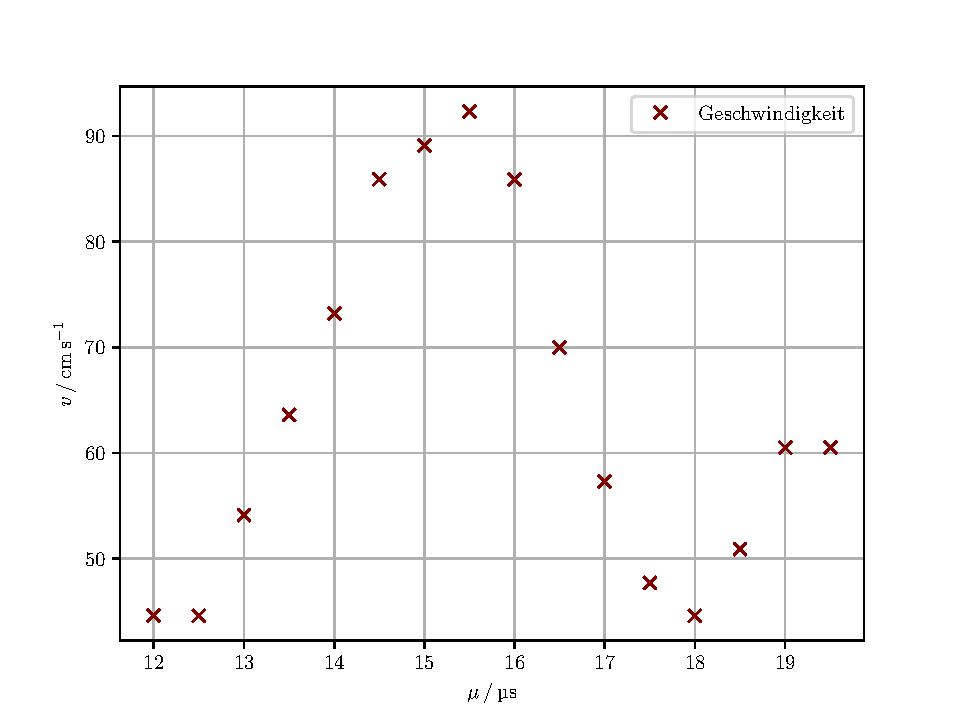
\includegraphics[height=5.5cm]{plots/70velocity.pdf}
        \caption{Die Geschwindigkeit.}
        \label{fig:70velo}
    \end{subfigure}
    \begin{subfigure}{0.48\textwidth}
        \centering
        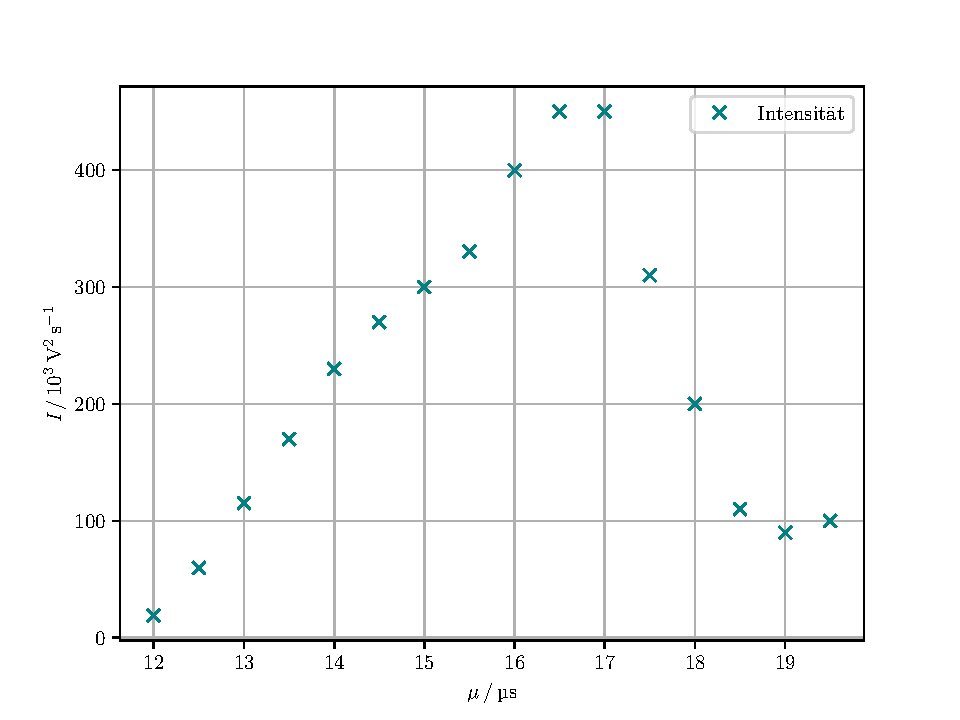
\includegraphics[height=5.5cm]{plots/70intensity.pdf}
        \caption{Die Streuintensität.}
        \label{fig:70inten}
    \end{subfigure}
    \caption{Die bei $70\,\%$ Pumpleistung aufgenommenen Messpunkte.}
    \label{fig:70vi}
\end{figure}

\begin{figure}
    \centering
    \begin{subfigure}{0.48\textwidth}
        \centering
        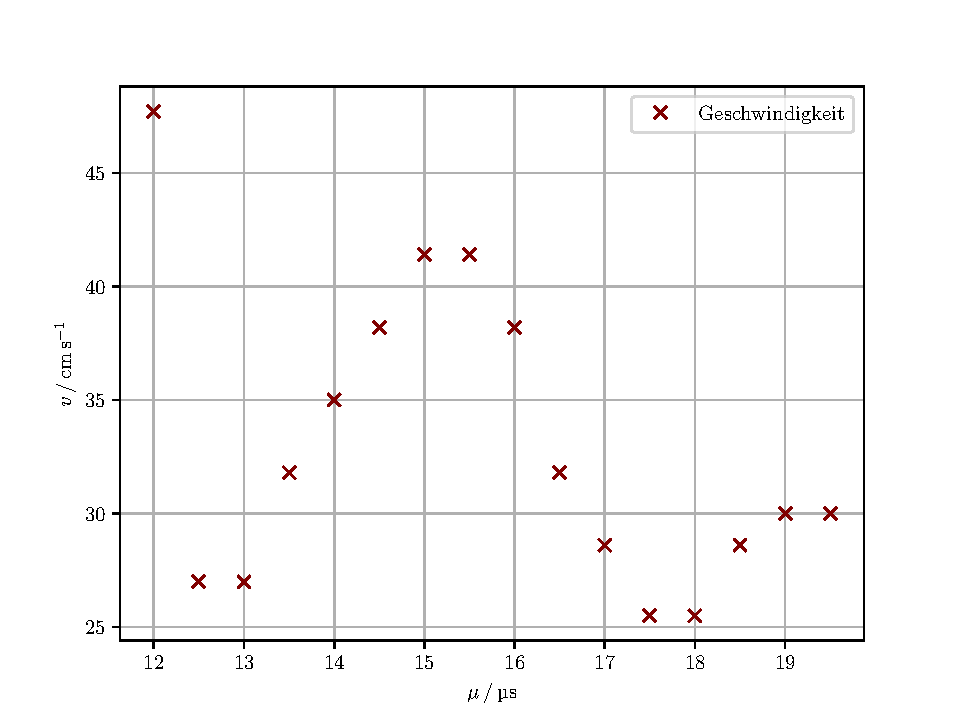
\includegraphics[height=5.5cm]{plots/45velocity.pdf}
        \caption{Die Geschwindigkeit.}
        \label{fig:45velo}
    \end{subfigure}
    \begin{subfigure}{0.48\textwidth}
        \centering
        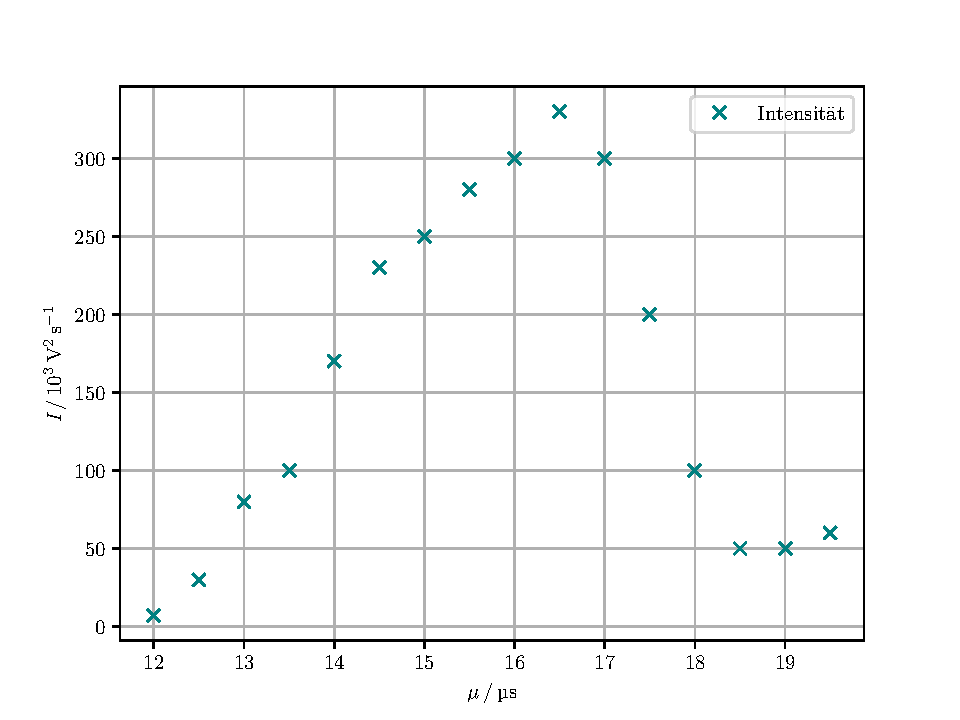
\includegraphics[height=5.5cm]{plots/45intensity.pdf}
        \caption{Die Streuintensität.}
        \label{fig:45inten}
    \end{subfigure}
    \caption{Die bei $45\,\%$ Pumpleistung aufgenommenen Messpunkte.}
    \label{fig:45vi}
\end{figure}

Das Strömungsprofil einer Röhre mit Radius $R$ ist gegeben durch 
\begin{equation}
    v(r)=v_\text{max}\cdot (1-\frac{r}{R})^{\sfrac{1}{n}}\,,
    \label{eqn:Geschwindigkeit}
\end{equation}
wobei $r$ den Abstand zur Symmetrieachse des Rohrs angibt (also immer $r>0$).
Ist die Strömung laminar (Reynoldszahl kleiner als etwa 2000), ist die Geschwindigkeitskurve parabelförmig, also $n=2$.
$n$ ist schwach von der Reynoldszahl abhängig; außerdem hat die Rauheit der Rohrinnenwand Einfluss auf die Größe der Zahl. 
Für eine sehr große Reynoldszahl $>\num{2e6}$ konvergiert der invertierte Exponent $n$ gegen $n=10$. 

Die Reynoldszahl einer Röhre berechnet sich über 
\begin{equation}
    Re=\frac{\rho v d}{\eta}\,,
\end{equation}
mit der Dichte $\rho$, der mittleren Geschwindigkeit $v$, der charakteristischen Länge $d$, die bei Rohren auf den Durchmesser festgelegt ist, 
sowie der dynamischen Viskosität $\eta$. 
Übersteigt die Reynoldszahl die kritische Reynoldszahl von etwa $2000$, ist die Strömung nicht mehr laminar, sondern turbulent. 

Wird für die gemittelte Geschwindigkeit jeweils die maximale Geschwindigkeit bei die Berechnung der Reynoldszahl verwendet, 
liegt die tatsächliche Reynoldszahl unter diesem Wert. 
Die Werte für diese obere Schranke sind in Tabelle \ref{tab:Reynoldszahl} aufgeführt. 
Es ist ersichtlich, dass die Strömungen in den Rohren wirklich laminar sind. 
Somit kann Gleichung \eqref{eqn:Geschwindigkeit} mit $n=2$ verwendet werden. 
\begin{table}
    \centering
    \caption{Obere Schranke für die Reynoldszahl der Strömungen.}
    \label{tab:Reynoldszahl}
    \begin{tabular}{c c c}
        \toprule
        Pumpleistung & $v_\text{max}\,/\,\si{\centi\meter\per\second}$ & $Re_\text{max}$ \\
        \midrule
        $70\,\%$ & 92.3 & 885 \\
        $45\,\%$ & 41.4 & 397 \\        
        \bottomrule
    \end{tabular}
\end{table}

Um ein Maß für die experimentelle Abweichung zu bekommen, wird mit der Methode der kleinsten Quadrate von \cite{scipy} 
die Gleichung \eqref{eqn:Geschwindigkeit} angenähert. 
Der Parameter $R$ wird vorgegeben mit der Hälfte des Rohrinnendurchmessers (vgl. Tabelle \ref{tab:techDaten}); außerdem wird die Messtiefe wieder in Längeneinheiten umgerechnet und der Definitionsbereich 
der Abszisse auf ein Intervall der Länge $2R$ so beschränkt, dass das Geschwindigkeitsmaximum in der Mitte liegt. 
Die Extremalstelle wird durch Vergleich der Abbildungen \ref{fig:70velo} und \ref{fig:45velo} auf $\mu_\text{max}=\SI{15.25}{\micro\second}$
bestimmt. 
Außerdem muss noch beachtet werden, dass das Argument $r$ per Definition immer positiv sein muss -- $r$ wird also durch $|r|$ ersetzt. 

Die entsprechenden Graphiken sind in Abbildung \ref{fig:str70} und \ref{fig:str45} zu finden. 
Die Geradenparameter sowie ihre relativen Abweichungen sind in Tabelle \ref{tab:Regr} zusammengefasst. 
\begin{figure}
    \centering
    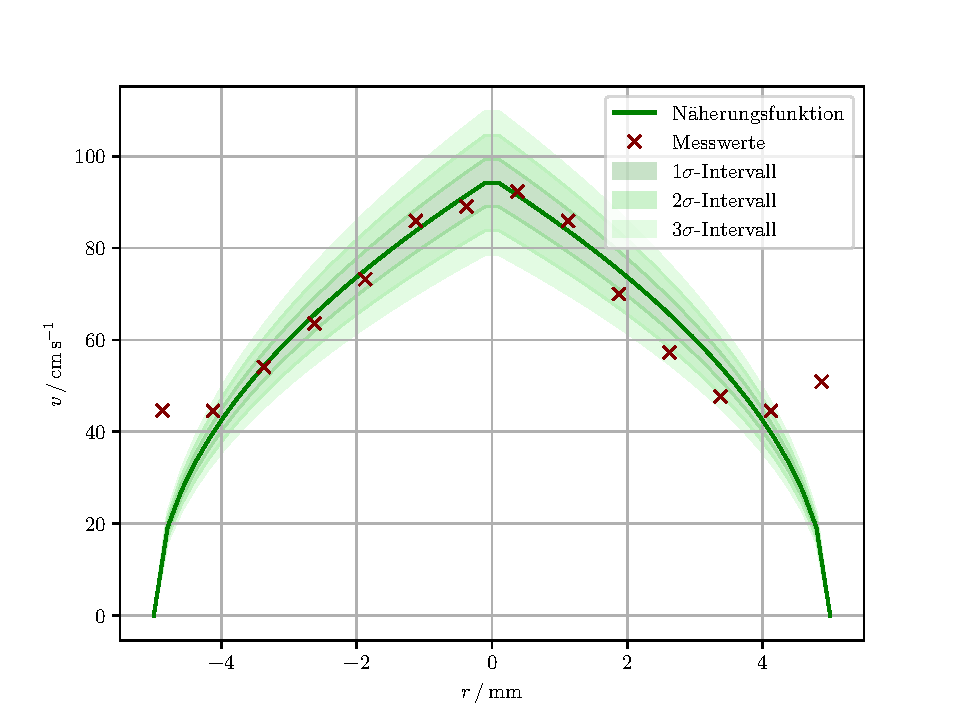
\includegraphics[width=0.8\textwidth]{plots/70regr.pdf}
    \caption{Regression des Strömungsprofils bei $70\,\%$ Leistung.}
    \label{fig:str70}
\end{figure}
\begin{figure}
    \centering
    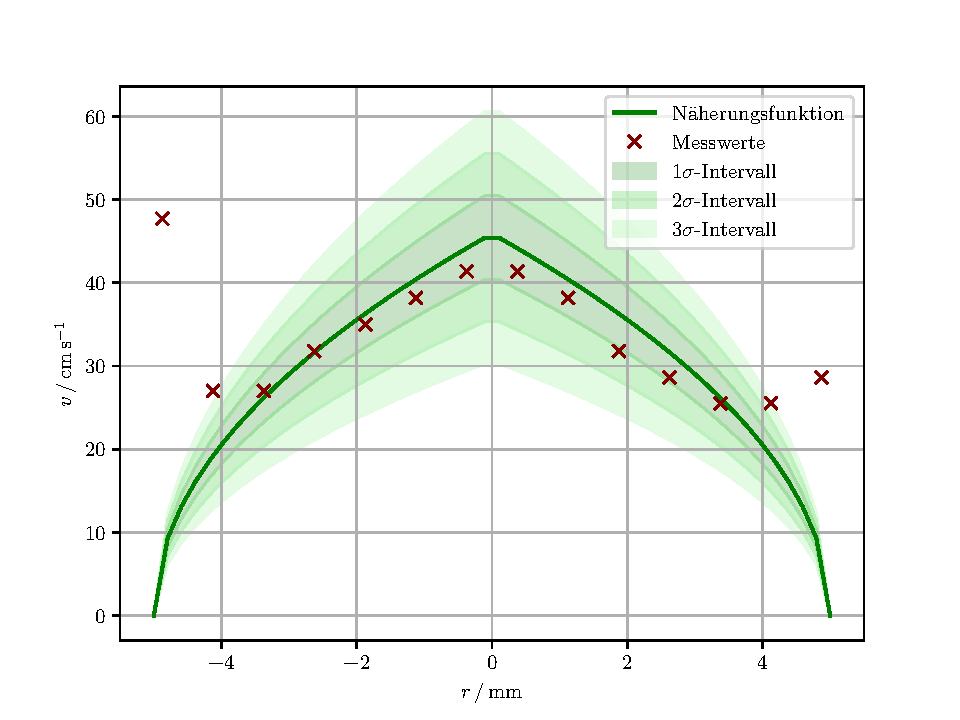
\includegraphics[width=0.8\textwidth]{plots/45regr.pdf}
    \caption{Regression des Strömungsprofils bei $45\,\%$ Leistung.}
    \label{fig:str45}
\end{figure}
\begin{table}
    \centering
    \caption{Die durch lineare Regression berechneten Maximalgeschwindigkeiten.}
    \label{tab:Regr}
    \begin{tabular}{c c c c}
        \toprule
        Leistung & $v_\text{max}\,/\,\si{\centi\meter\per\second}$ & $\Delta v_\text{max}\,/\,\si{\centi\meter\per\second}$ & relative Abweichung $\sfrac{\Delta v}{v}$ \\
        \midrule
        $70\,\%$ & 95.1 & 5.2 & $5.5\,\%$ \\
        $45\,\%$ & 45.9 & 5.1 & $11.1\,\%$ \\
        \toprule
    \end{tabular}
\end{table}